
The specific conductivity $\kappa$ of a solution describes the availability and capacity of movable charges within a substance. In the case of solutions, which were the focus of the experiments carried out, this refers to the ions of dissociated electrolytes. 

\begin{figure}[H]
    \centering
    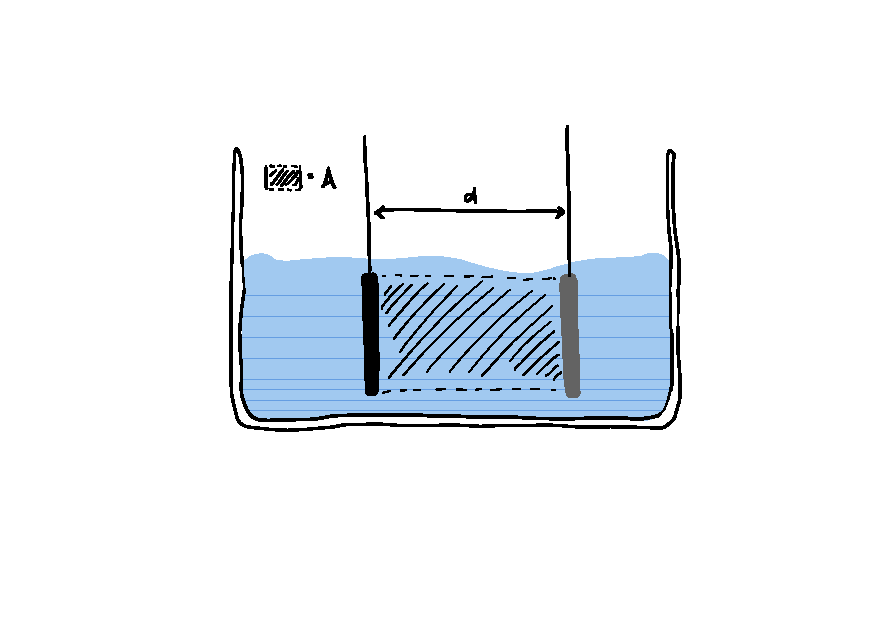
\includegraphics[width=.4\textwidth]{figures/Kappa.pdf}
    \label{fig:sketch_measuring}
    \caption{A schematic setup to measure the conductivity of a liquid.}
\end{figure}


Specific conductivity can be quantified by
\begin{equation} \label{eq:7.5}
    \kappa = \frac{d / A}{R}
\end{equation}

where $d$ is the distance between between two electrodes immersed in the solution, $A$ is the spanned cross sectional area. see fig and $R$ the electrical resistance. It is measured in Siemens $S$ which is equivalent to $1 / \Omega$.

As such, $\kappa$ correlates with how fast the available ions can move within the solution by: % hellooo :) super geschrieben die Einführung! helloooosies  danke :))) das results auch omg so professionell booooooah

\begin{equation} \label{eq:7.4}
    v_i = \frac{e E}{6 \pi \eta} \frac{z_i}{r_i}
\end{equation}

whereby $z_i * e$ is the respective ion's charge, $E$ is the electric field strength, $\eta$ is the viscosity coefficient and $r_i$ is the radius of the ion plus the solvent molecules surrounding it. It can be seen, that $v_i$ increases when $r_i$ or $\eta$ decreases.

This explains the correlation between temperature and conductivity, as the viscosity $\eta$ decreases when the temperature increases, causing $v_i$ and therefore $\kappa$ to increase as well.

Past empirical observations have shown, that within the range of several tens of degrees Celsius relative to a starting temperature $T_0$, changes in conductivity follow a linear model:

\begin{equation} \label{eq:7.6}
    \kappa(T) = \kappa(T_0)(1 + \alpha(T - T_0))
\end{equation}

where $\alpha$ is called temperature coefficient and can be calculated by: 

\begin{equation} \label{eq:7.7}
    \alpha = \frac{\mathrm{d}\kappa / \mathrm{d}T}{\kappa(T_0)}
\end{equation}

Furthermore, $\kappa$ also depends on the concentration of the given electrolyte within the solution. Intuitively, the more mobile charges are available, the higher the solution's conductivity will be. This holds especially true for diluted solutions of strong electrolytes (at constant temperature) where the correlation between conductivity $\kappa$ and concentration $c$ can be described approximately by 

\begin{equation} \label{eq:7.8}
    \kappa = \Lambda c
\end{equation}

where $\Lambda$ is called the molar conductivity and used to compare the conductivities of different electrolytes regardless of $c$.

However, when measuring molar conductivities accurately over a broad range of concentrations, it becomes clear that the molar conductivity varies slightly.

% However, the higher the concentration, the less accurate the model becomes due to increasing electrostatic interactions between the ions.

Here \textit{Kohlrausch's square root law} offers a more accurate mathematical model:

\begin{equation} \label{eq:kohlrausch}
    \Lambda = \Lambda_0 - k \sqrt{c}
\end{equation}

where $k$ is a constant dependant on the valency of the ions and $\Lambda^0$ is the extrapolated value generated by approximating $c=0$ called the limiting molar conductivity.

The overall conductivity of a solution containing more than one electrolyte depends on the respective electrolyte's conductivity as well as the ratio at which they are present within the solution. As such, changes to this ratio can result in changes to the overall conductivity as is utilized in conductometric titrations. 
















\iffalse{

In order to induce vaporization of a substance (the phase transition of liquid to gaseous \textit{at} boiling temperature\footnote{Not to confuse with evaporation, which is the phase transition \textit{below} the boiling temperature of a substance.}), heat must be provided to the system. Under the condition that vapor pressure $p$ and temperature $T$ remain constant during vaporization, the thermal energy provided to the system per mole of vaporized substance equals its molar enthalpy of vaporization $\Delta_VH$.

For the small temperature range of the experiments detailed further on, enthalpies of vaporization can be treated as material constants. Clausius-Clapeyron's model,

\begin{equation} \label{eq:6.2} %\tag{6.2}
    \frac{dp}{dT} = \frac{h^{(g)} - h^{(l)}}{T \space (v^{(g)} - v^{(l)})}
\end{equation}

where $h^{(\varphi)}$ and $v^{(\varphi)}$  are the molar volumes of the substance in its liquid and gaseous phases $\varphi$, treats vapor pressure as a function of boiling temperature $T$ with the coexistence curve between liquid and gaseous phases for a graph, and describes the change $dp$ expected for a variation of $dT$ in the substance’s boiling temperature.

Taking into account that $v^{(g)} >> v^{(l)}$, and provided the gaseous phase behaves according to ideal gas law 

\begin{equation} \label{eq:6.5} %\tag{6.5 ideal gas law}
    v^{(g)} = \frac{R T}{p}
\end{equation}

the differential equation can be simplified to

\begin{equation} \label{eq:6.6} %\tag{6.6}
    \frac{dp}{p} = \frac{\Delta_VH}{R} \frac{dT}{T^2}
\end{equation}

Integration yields

\begin{equation} \label{eq:6.7} %\tag{6.7}
    \ln \left( \frac{p}{p_0} \right) = \frac{\Delta_VH}{R} \left( \frac{1}{T_0} - \frac{1}{T} \right)
\end{equation}

Where $p_0$ and $T_0$ are atmospheric pressure and normal boiling temperature at atmospheric pressure respectively and $\Delta_VH$ can be calculated with an arbitrary point $(p, T)$ on the coexistence curve.


The substance’s entropy of vaporization at normal boiling temperature can be calculated via the Gibbs-Helmholtz equation 

%delta G = delta vh – T , 
\begin{equation}\label{eq:gibbs} %\tag{Gibbs-Helmholtz}
    \Delta G = \Delta_VH - T \Delta_VS
\end{equation}
% G = delta vh – T S
knowing that $\Delta G = 0$ for reactions that have reached an equilibrium.

A phase transitions from the liquid to the gaseous phase can also take place below boiling temperature and vapor pressure. This can be observed for example when blow-drying one’s hair or upon stepping out of the water as the droplets on the skin gradually evaporate. This is possible, because energy levels of the molecules inside the substance differ and some molecules have enough energy to overcome the threshold of the inter-molecular forces binding them to the liquid.

The molecule’s transition from fluid to gaseous phase requires energy which is taken from the fluid in the form of thermal energy, causing a momentary drop in temperature. If the fluid shares an interface with another substance (for example the skin) which has a higher temperature, it will in turn draw energy from this surface to compensate for the deficit.
Such changes in temperature are very minor for small volumes of evaporated liquid but can be measured for example if the interface is shared with a highly sensitive temperature sensor. 

The recorded temperature drops at contact with the sample and return to its previous value once the entire liquid has evaporated, presenting as a downward peak in a diagram where the sensor’s temperature is plotted against time. The area under the peak, established as $A$, which is calculated form the data obtained from the sensor, is proportional to the thermal energy taken by the liquid from the sensor during that time:

\begin{equation} \label{eq:6.15} %\tag{6.15}
    %A = k Q_V = k n \Delta_VH
    A = \int \Delta T dt \propto Q = n \Delta_VH
\end{equation}

where $n$ is the amount of substance given in moles.

The molar enthalpy of evaporation of the substance can be calculated from this using a reference substance with a known molar enthalpy of evaporation as follows:

\begin{equation} \label{eq:6.18} %\tag{6.18}
    \Delta_VH_{\text{subst}} = \Delta_VH_{\text{ref}} {\rho_{\text{ref}} \over \rho_{\text{subst}}} {M_{\text{subst}} \over M_{\text{ref}}} {A_{\text{subst}} \over A_{\text{ref}}}
\end{equation}

Where $\rho$ is the sample’s density, determined separately or taken from known literature.


}